% TODO checklist:
% - [x] Inspected src/jobs/models.py (JobDocument, JobStatus, SSEEvent, JobCreateRequest)
% - [x] Inspected src/jobs/interfaces.py (JobStore, IdempotencyStore, EventStore abstractions)
% - [x] Inspected src/jobs/factory.py (storage backend factory pattern)
% - [x] Inspected src/jobs/memory_store.py (in-memory implementations for testing)
% - [x] Inspected src/jobs/metrics.py (Prometheus instrumentation)
% - [x] Inspected db/redis_cache/job_store.py (Redis implementations)
% - [x] Inspected Q&A.md sections 38-41 for design rationale

\section{Asynchronous Job System}
\label{sec:job-system}

Enterprise AI agent platforms must handle workloads that exceed typical HTTP request timeouts. Training runs, batch processing, graph analytics, and multi-step agent executions can require minutes to hours of processing time. The Cineca Agentic Platform addresses this requirement through a comprehensive asynchronous job system that decouples job submission from execution, provides real-time progress updates, and ensures reliable completion even under adverse conditions.

This section presents the design and implementation of the job system, focusing on the domain model, lifecycle state machine, storage abstractions, and idempotency guarantees that enable robust long-running task execution.

\subsection{Design Goals and Requirements}

The asynchronous job system was designed to satisfy several key requirements derived from enterprise deployment scenarios:

\begin{enumerate}
    \item \textbf{Decoupled Execution}: Job submission must return immediately with a job identifier, allowing clients to poll for status or subscribe to event streams without blocking.
    
    \item \textbf{Multi-Tenant Isolation}: Jobs must be scoped to tenants and owners, with strict access control preventing cross-tenant visibility or manipulation.
    
    \item \textbf{Reliable State Tracking}: Job status transitions must be atomic and persistent, surviving process restarts and infrastructure failures.
    
    \item \textbf{Idempotent Submission}: Duplicate job submissions with the same parameters must return the existing job rather than creating duplicates.
    
    \item \textbf{Real-Time Progress}: Clients must receive timely updates on job progress through Server-Sent Events (SSE) with resume capability.
    
    \item \textbf{Graceful Cancellation}: Running jobs must support cooperative cancellation without resource leaks or inconsistent state.
    
    \item \textbf{Operational Visibility}: Comprehensive metrics must expose job throughput, latency distributions, and failure rates.
\end{enumerate}

\subsection{Job Lifecycle State Machine}

The job lifecycle follows a deterministic finite state machine with five states and well-defined transitions. Figure~\ref{fig:job-state-machine} illustrates the state diagram.

\begin{figure}[ht]
\centering
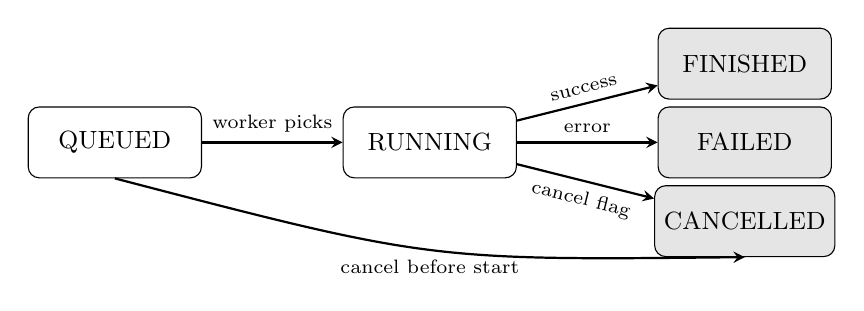
\begin{tikzpicture}[
    state/.style={rectangle, rounded corners, draw, minimum width=2.2cm, minimum height=0.9cm, font=\small},
    terminal/.style={rectangle, rounded corners, draw, fill=gray!20, minimum width=2.2cm, minimum height=0.9cm, font=\small},
    transition/.style={->, >=stealth, thick}
]
    % States
    \node[state] (queued) at (0,0) {QUEUED};
    \node[state] (running) at (4,0) {RUNNING};
    \node[terminal] (finished) at (8,1) {FINISHED};
    \node[terminal] (failed) at (8,0) {FAILED};
    \node[terminal] (cancelled) at (8,-1) {CANCELLED};
    
    % Transitions
    \draw[transition] (queued) -- node[above, font=\scriptsize] {worker picks} (running);
    \draw[transition] (running) -- node[above, font=\scriptsize, sloped] {success} (finished);
    \draw[transition] (running) -- node[above, font=\scriptsize] {error} (failed);
    \draw[transition] (running) -- node[below, font=\scriptsize, sloped] {cancel flag} (cancelled);
    \draw[transition] (queued.south) .. controls (4,-1.5) .. node[below, font=\scriptsize] {cancel before start} (cancelled.south);
\end{tikzpicture}
\caption{Job lifecycle state machine with terminal states (shaded).}
\label{fig:job-state-machine}
\end{figure}

The states and their semantics are defined as follows:

\begin{itemize}
    \item \textbf{QUEUED}: The job has been created and is waiting in the Redis queue for a worker to claim it. This is the initial state for all newly created jobs.
    
    \item \textbf{RUNNING}: A worker has dequeued the job and is actively executing it. Heartbeat timestamps are updated periodically to indicate worker liveness.
    
    \item \textbf{FINISHED}: The job completed successfully. The \texttt{result} field contains the output payload.
    
    \item \textbf{FAILED}: The job encountered an unrecoverable error. The \texttt{error} field contains the error message.
    
    \item \textbf{CANCELLED}: The job was cancelled by user request, either before execution started or during execution via cooperative cancellation.
\end{itemize}

The \texttt{JobStatus} enumeration in \texttt{src/jobs/models.py} implements this state machine with a helper property to identify terminal states:

\begin{lstlisting}[language=Python, caption={Job status enumeration with terminal state detection.}]
class JobStatus(str, Enum):
    """Job lifecycle states."""
    QUEUED = "queued"
    RUNNING = "running"
    FINISHED = "finished"
    FAILED = "failed"
    CANCELLED = "cancelled"

    @property
    def is_terminal(self) -> bool:
        """Check if this status is a terminal state."""
        return self in (JobStatus.FINISHED, 
                        JobStatus.FAILED, 
                        JobStatus.CANCELLED)
\end{lstlisting}

\subsection{Job Document Structure}
\label{subsec:job-document-structure}

The \texttt{JobDocument} model represents the core job entity, designed to be storage-agnostic while supporting serialization to both Redis HASH structures and PostgreSQL rows. Table~\ref{tab:job-document-fields} describes each field.

\begin{table}[ht]
\centering
\caption{JobDocument schema fields and their purposes.}
\label{tab:job-document-fields}
\small
\begin{tabular}{llp{6.5cm}}
\hline
\textbf{Field} & \textbf{Type} & \textbf{Description} \\
\hline
\texttt{id} & UUID (string) & Unique job identifier, generated on creation \\
\texttt{owner} & string & Owner subject extracted from JWT \texttt{sub} claim \\
\texttt{tenant\_id} & string & Tenant isolation boundary for multi-tenancy \\
\texttt{type} & string & Job type (e.g., \texttt{demo}, \texttt{test}, \texttt{long-running}, \texttt{agent.run}) \\
\texttt{status} & JobStatus & Current lifecycle state \\
\texttt{payload} & JSON object & Job-specific input parameters \\
\texttt{result} & JSON object & Job output, populated on successful completion \\
\texttt{error} & string & Error message if status is FAILED \\
\texttt{created\_at} & ISO8601 datetime & Job creation timestamp (UTC) \\
\texttt{updated\_at} & ISO8601 datetime & Last status change timestamp (UTC) \\
\hline
\end{tabular}
\end{table}

The model provides bidirectional serialization methods for Redis HASH storage:

\begin{lstlisting}[language=Python, caption={JobDocument serialization for Redis storage.}]
def to_hash_dict(self) -> dict[str, str]:
    """Convert to flat string dict for Redis HASH storage."""
    return {
        "id": self.id,
        "owner": self.owner,
        "tenant_id": self.tenant_id,
        "type": self.type,
        "status": self.status.value,
        "payload": json.dumps(self.payload),
        "result": json.dumps(self.result) if self.result else "",
        "created_at": self.created_at.isoformat(),
        "updated_at": self.updated_at.isoformat() if self.updated_at else "",
        "error": self.error or "",
    }

@classmethod
def from_hash_dict(cls, data: dict[str, str | bytes]) -> JobDocument:
    """Reconstruct from Redis HASH."""
    # Handle both str and bytes (Redis client variations)
    def decode(v): return v.decode("utf-8") if isinstance(v, bytes) else v
    # ... parsing logic
\end{lstlisting}

\subsection{Job Type Registry}

The platform supports multiple job types, each with distinct execution semantics. The allowed types are configured via the \texttt{ALLOWED\_JOB\_TYPES} setting, with defaults including:

\begin{itemize}
    \item \textbf{demo}: Simple sleep-based simulation for testing, with configurable duration via \texttt{duration\_ms} payload parameter.
    
    \item \textbf{test}: Instant completion with payload echo, useful for integration testing.
    
    \item \textbf{long-running}: Multi-step execution with configurable step count and periodic progress updates.
    
    \item \textbf{agent.run}: Full agent orchestration execution via Workflow B (see Section~\ref{subsubsec:workflow-b}), providing complete orchestrator integration with PII scrubbing, output guards, and real-time SSE progress streaming.
\end{itemize}

The \texttt{agent.run} job type represents the production use case for asynchronous agent execution, enabling fault-tolerant orchestration that survives API server restarts and supports horizontal scaling of worker processes.

\subsection{Storage Abstraction Layer}

The job system employs a repository pattern with abstract interfaces, enabling pluggable storage backends. Three interfaces define the contract:

\subsubsection{JobStore Interface}

The \texttt{JobStore} abstract base class defines operations for job document persistence:

\begin{lstlisting}[language=Python, caption={JobStore interface for job persistence.}]
class JobStore(ABC):
    @abstractmethod
    async def create(self, job: JobDocument, ttl_seconds: int) -> None:
        """Persist a new job with automatic expiry."""
        pass

    @abstractmethod
    async def get(self, job_id: str) -> JobDocument | None:
        """Retrieve job by ID, None if expired/not found."""
        pass

    @abstractmethod
    async def update_status(
        self, job_id: str, status: JobStatus,
        result: dict | None = None, error: str | None = None,
        ttl_seconds: int | None = None,
    ) -> bool:
        """Atomically update job status and optional result/error."""
        pass

    @abstractmethod
    async def list_by_owner(
        self, owner: str, status: JobStatus | None = None,
        offset: int = 0, limit: int = 25,
    ) -> tuple[list[JobDocument], int]:
        """List jobs for owner, newest first, with pagination."""
        pass

    @abstractmethod
    async def delete(self, job_id: str) -> bool:
        """Delete job and all associated indices."""
        pass
\end{lstlisting}

\subsubsection{IdempotencyStore Interface}

The \texttt{IdempotencyStore} manages idempotency keys for duplicate request detection:

\begin{lstlisting}[language=Python, caption={IdempotencyStore interface for request deduplication.}]
class IdempotencyStore(ABC):
    @abstractmethod
    async def get_job_id(self, key: str) -> str | None:
        """Check if key exists and return associated job_id."""
        pass

    @abstractmethod
    async def store(self, key: str, job_id: str, ttl_seconds: int) -> None:
        """Store idempotency key with expiry."""
        pass
\end{lstlisting}

\subsubsection{EventStore Interface}

The \texttt{EventStore} manages the SSE event ring buffer for real-time updates:

\begin{lstlisting}[language=Python, caption={EventStore interface for SSE event management.}]
class EventStore(ABC):
    @abstractmethod
    async def append(self, job_id: str, event: SSEEvent, ring_size: int) -> None:
        """Append event to ring buffer, capping at ring_size."""
        pass

    @abstractmethod
    async def get_next_event_id(self, job_id: str) -> int:
        """Get next monotonic event ID for this job."""
        pass

    @abstractmethod
    async def replay_from(self, job_id: str, last_event_id: int) -> list[SSEEvent]:
        """Retrieve events with event_id > last_event_id."""
        pass
\end{lstlisting}

\subsection{Storage Backend Implementations}

\subsubsection{Redis Backend (Production)}

The Redis implementation uses purpose-built data structures for optimal performance:

\begin{itemize}
    \item \textbf{Job Documents}: Stored as HASH at \texttt{job:\{id\}} with field-level access and TTL-based auto-expiry.
    
    \item \textbf{Global Index}: ZSET at \texttt{jobs:all} with score = created\_at epoch milliseconds for time-ordered pagination.
    
    \item \textbf{Owner Index}: ZSET at \texttt{jobs:owner:\{owner\}} for user-specific job listing.
    
    \item \textbf{Status Index}: ZSET at \texttt{jobs:status:\{status\}} for status-filtered queries.
    
    \item \textbf{Event Ring}: LIST at \texttt{job:\{id\}:events} with LPUSH + LTRIM for bounded storage.
    
    \item \textbf{Event Counter}: String at \texttt{job:\{id\}:event\_seq} for monotonic event IDs via INCR.
    
    \item \textbf{Idempotency Keys}: String at \texttt{idem:\{owner\}:\{tenant\}:\{type\}:\{hash\}:\{key\}} with 24-hour TTL.
\end{itemize}

The Redis implementation uses Lua scripts for atomic operations requiring multiple commands:

\begin{lstlisting}[language=Python, caption={Atomic job cancellation using Lua script.}]
async def cancel_job_atomic(self, job_id: str) -> bool:
    """Atomically cancel using Lua CAS (Compare-And-Set)."""
    await self._ensure_scripts_loaded()
    redis = await get_async_redis()
    
    result = await redis.evalsha(
        self._cancel_job_sha,
        1,  # numkeys
        f"job:{job_id}",  # KEYS[1]
        datetime.utcnow().isoformat(),  # timestamp
        json.dumps({"cancelled": True}),  # result
    )
    
    return result.decode("utf-8") == "cancelled"
\end{lstlisting}

\subsubsection{In-Memory Backend (Development/Testing)}

The in-memory implementation wraps Python dictionaries, providing identical API semantics without external dependencies:

\begin{lstlisting}[language=Python, caption={In-memory job store for testing.}]
_JOBS: dict[str, dict[str, Any]] = {}
_IDEMPOTENCY_KEYS: dict[str, str] = {}
_EVENTS: dict[str, list[SSEEvent]] = {}
_EVENT_SEQ: dict[str, int] = {}

class MemoryJobStore(JobStore):
    def __init__(self):
        self._jobs = _JOBS

    async def create(self, job: JobDocument, ttl_seconds: int) -> None:
        """Store job in memory (TTL ignored)."""
        self._jobs[job.id] = {...}  # Convert to dict
\end{lstlisting}

\subsection{Storage Backend Factory}

The factory pattern enables runtime selection of storage backends via configuration:

\begin{lstlisting}[language=Python, caption={Storage backend factory function.}]
def get_stores() -> tuple[JobStore, IdempotencyStore, EventStore]:
    """Factory for job storage backends based on configuration."""
    backend = settings.JOB_STORE_BACKEND.lower()

    if backend == "memory":
        logger.info("Using in-memory job storage (no TTL)")
        return (
            MemoryJobStore(),
            MemoryIdempotencyStore(),
            MemoryEventStore(ring_size=settings.SSE_RING_SIZE),
        )

    elif backend == "redis":
        from db.redis_cache.job_store import (
            RedisEventStore, RedisIdempotencyStore, RedisJobStore,
        )
        logger.info(f"Using Redis (TTL={settings.JOB_TTL_DAYS} days)")
        return (
            RedisJobStore(),
            RedisIdempotencyStore(),
            RedisEventStore(ring_size=settings.SSE_RING_SIZE),
        )

    raise ValueError(f"Invalid JOB_STORE_BACKEND: {backend}")
\end{lstlisting}

\subsection{Idempotency Mechanism}

Idempotent job creation prevents duplicate jobs from network retries or client errors. The idempotency key is computed from request context:

\begin{lstlisting}[language=Python, caption={Idempotency key generation algorithm.}]
def create_idempotency_key(
    owner: str, tenant: str, job_type: str,
    payload: dict, idempotency_key: str | None = None,
) -> str:
    """Generate idempotency key from request context."""
    # Hash payload for deterministic key generation
    payload_str = json.dumps(payload, sort_keys=True, separators=(",", ":"))
    payload_hash = hashlib.sha256(payload_str.encode()).hexdigest()[:16]
    
    key_suffix = idempotency_key or payload_hash
    return f"idem:{owner}:{tenant}:{job_type}:{payload_hash}:{key_suffix}"
\end{lstlisting}

The creation flow implements two-tier idempotency checking:

\begin{enumerate}
    \item \textbf{Redis Cache Check}: Fast lookup in idempotency store for recent duplicates.
    \item \textbf{PostgreSQL Authoritative Check}: If Redis misses, query PostgreSQL for the canonical job state.
    \item \textbf{Store Key}: On new job creation, store the idempotency key with 24-hour TTL.
\end{enumerate}

\subsection{Job Metrics Instrumentation}

Comprehensive Prometheus metrics provide operational visibility into job system performance:

\begin{lstlisting}[language=Python, caption={Job metrics definitions.}]
# Operation counters
job_create_total = Counter(
    "job_create_total", "Total job creations",
    ["backend", "status"]  # status: success, idempotent_replay, failed
)

job_get_total = Counter(
    "job_get_total", "Total job retrievals",
    ["backend", "status"]  # status: hit, miss
)

# Latency histograms
job_create_duration_seconds = Histogram(
    "job_create_duration_seconds", "Job creation latency",
    ["backend"],
    buckets=(0.001, 0.005, 0.010, 0.025, 0.050, 0.100, 0.250, 0.500, 1.0, 2.5, 5.0)
)

# SSE connection tracking
sse_connections_active = Gauge(
    "sse_connections_active", "Active SSE connections", ["backend"]
)

sse_resume_hits_total = Counter(
    "sse_resume_hits_total", "Successful Last-Event-ID resumes", ["backend"]
)
\end{lstlisting}

Decorator-based instrumentation wraps store operations:

\begin{lstlisting}[language=Python, caption={Metrics tracking decorator.}]
def track_job_create(backend: str):
    """Decorator to track job creation metrics."""
    def decorator(func):
        @wraps(func)
        async def wrapper(*args, **kwargs):
            start = time.time()
            status = "failed"
            try:
                result = await func(*args, **kwargs)
                status = "success"
                return result
            finally:
                duration = time.time() - start
                job_create_duration_seconds.labels(backend=backend).observe(duration)
                job_create_total.labels(backend=backend, status=status).inc()
        return wrapper
    return decorator
\end{lstlisting}

\subsection{Configuration Parameters}

Table~\ref{tab:job-config} summarizes the configurable parameters for the job system.

\begin{table}[ht]
\centering
\caption{Job system configuration parameters.}
\label{tab:job-config}
\small
\begin{tabular}{lll}
\hline
\textbf{Parameter} & \textbf{Default} & \textbf{Description} \\
\hline
\texttt{JOB\_STORE\_BACKEND} & \texttt{memory} & Storage backend (\texttt{memory}, \texttt{redis}) \\
\texttt{JOB\_TTL\_DAYS} & 10 & Job document TTL in days \\
\texttt{SSE\_RING\_SIZE} & 100 & Maximum events in ring buffer \\
\texttt{IDEMPOTENCY\_TTL\_HOURS} & 24 & Idempotency key expiration \\
\texttt{ALLOWED\_JOB\_TYPES} & \texttt{demo,test,long-running} & Permitted job types \\
\hline
\end{tabular}
\end{table}

